\documentclass{beamer}

% preamble speciale Jacob Harder
% 31. jan. 2020

%packages

\usepackage[utf8]{inputenc} %utf8 is probably good
\usepackage{amsmath}
\usepackage{amssymb}
\usepackage{amsthm}
\usepackage{graphicx} %for including images
\usepackage{float} %for exact placement of figure (and more?)
\usepackage{mathtools} %for \mathclap (stacking under sums)
\usepackage{dsfont} %for boldface numbers
\usepackage{bm} %vectors in bold
\usepackage[ruled,vlined]{algorithm2e}
\usepackage{cleveref}
\usepackage{ifthen}
\usepackage{commath}
\usepackage[a4paper,width=150mm,top=25mm,bottom=25mm]{geometry}
\usepackage{upgreek}
%\usepackage[inline]{enumitem}
\usepackage{multicol}
%\usepackage{fancyhdr} %maybe later..
%\pagestyle{fancy}
\usepackage{mathabx}
\usepackage{csquotes}
\usepackage{tikz}
\usepackage{outline} %for subitems in lists

%front page
\usepackage{wallpaper}
\usepackage{titling}

%bibliography
\usepackage[numbers]{natbib}
\bibliographystyle{plainnat}
\newcommand{\mcite}[1]{[\citenum{#1}, \citeauthor{#1} (\citeyear{#1})]}
\newcommand{\ncite}[1]{\cite{#1}}

%linespread and geometry
\linespread{1.3}

%commands
\newcommand{\Cal}{\mathcal}
\newcommand{\cl}{\mathcal}
\newcommand{\fk}{\mathfrak}
\newcommand{\bb}{\mathbb}
\newcommand{\Q}{\bb{Q}}
\newcommand{\Z}{\bb{Z}}
\newcommand{\N}{\bb{N}}
\newcommand{\R}{\bb{R}}
\newcommand{\C}{\bb{C}}
\newcommand{\E}{\bb{E}}
\newcommand{\Rext}{\ol{\ul{\R}}}
\newcommand{\Var}{\mathrm{Var}}
\newcommand{\Prob}{\mathds{P}} %fundamental probability measure
\newcommand{\idc}{\mathds{1}}
\newcommand{\ve}{\varepsilon} %abbreviation for epsilon
\newcommand{\Yp}{\Upupsilon} %abbreviation for Ypsilon
\newcommand{\difd}{\; \mathrm{d}} %differential d
\newcommand{\wt}{\widetilde}
\newcommand{\wh}{\widehat}
\newcommand{\ol}{\overline}
\newcommand{\ul}{\underline}
\newcommand{\Mid}{\;\middle\vert\;}
\newcommand{\id}{\text{id}}
\newcommand{\supp}{\text{supp}}
\newcommand{\defemph}[1]{\textbf{#1}} %first-mentions of names
\DeclarePairedDelimiter\ceil{\lceil}{\rceil}
\DeclarePairedDelimiter\floor{\lfloor}{\rfloor}
\DeclareMathOperator*{\argmax}{argmax}
\DeclareMathOperator*{\argmin}{argmin}
\newcommand{\defeq}{\vcentcolon=} %definition equality symbol
%add single eq. tag in align*
\newcommand\numberthis{\addtocounter{equation}{1}\tag{\theequation}}
\newcommand{\rleft}[1]{\rotatebox[origin=c]{90}{\ensuremath{#1}}}
\newcommand{\vrel}[3]{ % for vertical subseteq e.g.
\vcenter{\halign{\hfill##\hfill\cr
\ensuremath{#1}\cr
\rotatebox[origin=c]{270}{\ensuremath{#2}}\cr
\ensuremath{#3}\cr
}}}
\newcommand{\lar}{\leftrightarrow}
\newcommand{\Span}{\mathrm{span}}
\newcommand{\Gr}{\mathrm{Gr}}

%theorems
\theoremstyle{definition}
\newtheorem{thm}{Theorem}[chapter]
\newtheorem{lem}[thm]{Lemma}
\newtheorem{defn}[thm]{Definition}
\newtheorem{cor}[thm]{Corollary}
\newtheorem{rem}[thm]{Remark}
\newtheorem{prop}[thm]{Proposition}
\newtheorem{asm}{Assumption}
\newtheorem{example}[thm]{Example}
%\newtheorem{cond}{Condition}
\newtheorem{sett}{Setting}
\newtheorem{innercond}{Condition}
\newenvironment{cond}[1]
  {\renewcommand\theinnercond{#1}\innercond}
  {\endinnercond}

%cref
\crefname{algocf}{alg.}{algs.}
\Crefname{algocf}{Algorithm}{Algorithms}
\crefname{innercond}{}{}
\Crefname{innercond}{}{}



\begin{document}

\begin{frame}
	\frametitle{Markov decision process}
	\begin{Defi}
		A Markov decision process (MDP) $(\Cal{S}, \Cal{A}, P, R, \gamma)$
		consists of
		\begin{itemize}
			\item $\Cal{S}$ a set of states (in my case $\subseteq \R^n$)
			\item $\Cal{A}$ a set of actions (in my case \emph{finite})
			\item $P : \Cal{S} \times \Cal{A} \to \Cal{P}(\Cal{S})$
				its Markov transition kernel
			\item $R : \Cal{S} \times \Cal{A} \to \Cal{P}(\R)$
				its immediate reward distribution
			\item $\gamma \in (0,1)$ the discount factor
		\end{itemize}
	\end{Defi}

\end{frame}

\begin{frame}
	\frametitle{Q-Learning}
	\begin{itemize}
		\item Policy: $\pi : \Cal{S} \to \Cal{P}(\Cal{A})$
		\item State-value function: $V^\pi : \Cal{S} \to \R$
			\resizebox{\textwidth}{!}{ $V^\pi(s)
			= \E \left( \sum_{t \geq 0} \gamma^t R_t 
			\mid R_t \sim R(S_t, A_t), S_t \sim P(S_{t-1}, A_{t-1}), A_t
			\sim \pi(S_t), S_0 = s \right) $ }
		\item State-action-value (Q-) function $Q^\pi : \Cal{S} \times \Cal{A} \to \R$
			\[ Q^\pi(s, a) = \E (R(s, a) + \gamma V^\pi(S_0) \mid S_0 \sim P(s, a)) \]
		\item Optimal Q-function is defined as
			\[ Q^*(s, a) = \sup_\pi Q^\pi(s, a) \]
		\item One can show that there is a policy $\pi^*$ such that $Q^* = Q^{\pi^*}$.
			This is the optimal policy - the goal of Q-learning
			(and Reinforcement Learning in general). 
	\end{itemize}
\end{frame}

\begin{frame}
	\frametitle{Artificial Neural Networks}
	\begin{Definition}
	An \textbf{ANN} (Artificial Neural Network) with structure
	$\{ d_i \}_{i=0}^{L+1} \subseteq \N$,
	activation functions $\sigma_i = (\sigma_{ij} : \R \to \R)_{j=1}^{d_i}$
	and weights $\{ W_i \in M^{d_i \times d_{i-1}}, v_i \in \R^{d_i} \}_{i=1}^{L+1}$
	is the function $F:\R^{d_0} \to \R^{d_{L+1}}$ 
	\[ F(x) = w_{L+1} \circ \sigma_L \circ w_L \circ \sigma_{L-1} \circ \dots \circ w_1 x \]
		where $w_i$ is the affine function $x \mapsto W_i x + v_i$ for $i \in [L+1]$.

	Here $\sigma_i(x_1, \dots, x_{d_i})
	= (\sigma_{i1}(x_1), \dots, \sigma_{id_{i}}(x_{d_{i}}))$.

	$L \in \N_0$ is called the number of hidden layers.

	$d_i$ is the number of neurons or nodes in layer $i$.
	\end{Definition}

	An ANN is called \emph{deep} if there are two or more hidden layers.
\end{frame}

\begin{frame}
	\frametitle{The Bellman operator}
	Denote $\pi_Q$ as  the \emph{greedy} policy 
	with respect to $Q$ i.e. $\pi(s,a) = 1$ for $a = \argmax_a Q(s,a)$.
	For every policy $\pi$ we define the operators
	\[ (P^\pi Q)(s, a) = \E (Q(S', A') \mid S' \sim P(s, a), A' \sim \pi(S')) \]
	\[ (T^\pi Q)(s, a) = \E R(s, a) + \gamma (P^\pi Q)(s, a) \]
	$T^\pi$ is called the Bellman operator.
	It can be shown that $Q^{\pi}$ is a fixed point for $T^\pi$.
	Finally we define \emph{Bellmans optimality operator} $T$ as
	\[ T Q = T^{\pi_Q} Q \]
	Bellmans optimality equation is then $T Q^* = Q^*$.
\end{frame}

\begin{frame}
	\frametitle{Context}
	\begin{Theorem}
		If both $\Cal{S}$ and $\Cal{A}$ are finite,
		and $R$ is deterministic, then the simple iteration
		\[ Q_{t+1}(s_t, a_t) = Q_t(s_t, a_t) + \alpha_t(s_t, a_t)
			[R_t + \gamma Q_t(s_{t+1}, \pi_{Q_t}(s_{t+1})) - Q_t(s_t, a_t)] \]
		converges with probability 1 to $Q^*$, given that
		\[ \sum_{t\geq 1} \alpha_t(s, a) = \infty, \qquad
			\sum_{t\geq 1} \alpha^2_t(s, a) < \infty \]
		for all $(s, a) \in \Cal{S} \times \Cal{A}$.
	\end{Theorem}

	\begin{Theorem}[Universal approximation theorem]
		An ANN with 1 hidden layer is sufficient to approximate any continuous
		function $[0,1]^k \to \R$ (at cost of layer-width).
	\end{Theorem}
\end{frame}

\begin{frame}
	\frametitle{Sparse ReLU Network}
	\begin{definition}
		For $s,V \in \R$ a (s,V)-\textbf{Sparse ReLU Network} is an ANN $f$
		with any structure $\{d_i\}_{i\in [L+1]}$,
		all activation functions being \emph{ReLU} i.e. $\sigma_{ij} = \max(\cdot, 0)$
		and any weights $(W_\ell, v_\ell)$
		satisfying
		\begin{itemize}
			\item $\max_{\ell \in [L+1]} \norm{\widetilde{W}_\ell}_\infty \leq 1$
			\item $\sum_{\ell = 1}^{L+1} \norm{\widetilde{W}_\ell}_0 \leq s$
			\item $\max_{j \in [d_{L+1}]} \norm{f_j}_\infty \leq V$
		\end{itemize}
		Here $\widetilde{W}_\ell = (W_\ell, v_\ell)$.

		The set of them we denote $\Cal{F}(s,V)$.
	\end{definition}
\end{frame}

\begin{frame}
	\frametitle{The algorithm}
	\begin{algorithm}[H]
		\caption{Fitted Q-Iteration Algorithm}
		\KwIn{MDP $(\Cal{S}, \Cal{A}, P, R, \gamma)$, function class $\Cal{F}$,
			sampling distribution $\nu$, number of iterations $K$,
			number of samples $n$, initial estimator $\widetilde{Q}_0$}
		\For{$k = 0,1,2,\dots,K-1$}{
			Sample i.i.d. observations $\{(S_i, A_i), i \in [n]\}$ from $\nu$
			obtain $R_i \sim R(S_i, A_i)$ and $S'_i \sim P(S_i, A_i)$ \\
			Let $Y_i = R_i + \gamma \cdot \max_{a \in \Cal{A}} \widetilde{Q}_k(S'_i, a)$ \\
			Update action-value function:
			\[ \widetilde{Q}_{k+1} \leftarrow
				\argmin_{f \in \Cal{F}} \frac{1}{n}
				\sum_{i=1}^n (Y_i - f(S_i, A_i))^2 \]
		}
		Define $\pi_K$ as the greedy policy w.r.t. $\widetilde{Q}_K$ \\
		\KwOut{An estimator $\widetilde{Q}_K$ of $Q^*$ and policy $\pi_K$}
	\end{algorithm}
\end{frame}

\begin{frame}
	\frametitle{The theorem}
	For any $K \in \N$ let $Q^{\pi_K}$ be the action-value function
	corresponding to policy $\pi_K$ which is return by Algorithm 1,
	when run with a sparse ReLU network on the form
	\[ \Cal{F}_0 = \{f(\cdot, a) \in \Cal{F}(L^*, \{d_j^*\}_{j=0}^{L^*+1},s^*)
		\mid a \in \Cal{A} \} \]
	where
	\[ L^* \lesssim (\log n)^{\xi'}, d_0 = r, d_j^*, d_{L+1}=1, \lesssim n^{\xi'},
		s^* \asymp n^{\alpha^*} \cdot (\log n)^{\xi'} \]
	Let $\mu$ be any distribution over $\Cal{S} \times \Cal{A}$.
	Under \emph{some assumptions} 
	\\~\\
	\resizebox{\textwidth}{!}{ 
		$ \norm{Q^* - Q^{\pi_K}}_{1,\mu} \leq C \cdot \frac{\phi_{\mu,\nu}
			\cdot \gamma}{(1-\gamma)^2}
			\cdot |\Cal{A}| \cdot (\log n)^{\xi^*} \cdot n^{(\alpha^* - 1)/2} 
			+ \frac{4 \gamma^{K+1}}{(1-\gamma)^2} \cdot R_{\max} $ }
	\\~\\
	Here $\alpha^* \in (0,1), C, \xi', \xi^*, \phi_{\mu,\nu} \in \R_{+}$
	are constants depending on the assumptions
	and $R_{\max}$ the maximum possible reward.
\end{frame}

\begin{frame}
	\frametitle{Naive interpretation}
	This paper shows that for \emph{any} MDP satisfying mild(?) assumptions,
	its optimal policy $\pi^*$ can be approximated arbitrarily close by
	the fitted Q-iteration algorithm
	(in $\norm{\cdot}_1$ over the chosen $\mu$ distribution).
	I.e. this algorithm 'solves' (up to any precision)
	a large class of games, decision processes, etc.
	\begin{figure}
		\centering
		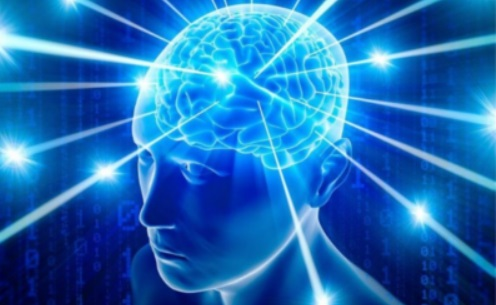
\includegraphics[scale=0.5]{Brain.jpg}
	\end{figure}
\end{frame}

\begin{frame}
	\frametitle{Problems}
	\begin{outline}
		\1 Are the assumptions actually mild?
		\1 How large are the constants / how quick is convergence?
		\1 In the algorithm we assumed that we could solve a least squares problem
			on a function class of Neural Networks with several restrictions.
			According to one reviewer this is an NP-hard problem.
		\1 Our result depended on a distribution $\mu$, so it does not say much
			about how close we are to $\pi^*$ outside the support of $\mu$.
		\1 The fitted Q-iteration algorithm differs from
			normal Deep Q-Learning in two important ways:
			\2 It avoids analysing errors in SGD and Back-Propagation 
			by assuming that a global optimum is found.
			\2 It uses a fixed distribution on $\Cal{S}\times{A}$ for batch sampling
			during \emph{experience replay} rather than picking
			uniformly from actual experiences.
	\end{outline}
\end{frame}


\begin{frame}
	\frametitle{Hölder Smoothness}
	\begin{Defi}
		Let $\Cal{D}\subseteq \R^r$ be compact and $\beta,H>0$. A function $f:\Cal{D}\to \R$
		we call Hölder smooth if
		\[ \sum_{{\alpha} : |{\alpha}| < \beta}
			\norm{\partial^{\alpha}f}_\infty +
			\sum_{{\alpha} : \norm{{\alpha}}_1 = \floor{\beta}}
			\sup_{x \neq y} \frac{|\partial^\alpha (f(x) - f(y))|}
			{\norm{x-y}_\infty^{\beta-\floor{\beta}}} \leq H \] 
		Where $\alpha = (\alpha_1, \dots, \alpha_r) \in \N^r$.
		We write $f \in C_r(\Cal{D}, \beta, H)$.
	\end{Defi}
	We consider families of \emph{Compositions of Hölder Functions}
	\[ \Cal{G}(\{p_j, t_j, \beta_j, H_j\}_{j \in [q]}) \]
	where $t_j, p_j \in \N$, $t_j\leq p_j$ and $H_j, \beta_j > 0$,
	defined as containing $f$ when $f = g_q \circ \dots \circ g_1$
	for $g_j : [a_j, b_j]^{p_j} \to [a_{j+1}, b_{j+1}]^{p_{j+1}}$
	functions on some real hypercubes that only depend on $t_j$ of their inputs
	for each of their components $g_{jk}$,
	and satisfies $g_{jk} \in C_{t_j}([a_j, b_j]^t_j, \beta_j, H_j)$.
\end{frame}

\begin{frame}
	\frametitle{Assumption 1, Hölder smoothness of $\Cal{F}_0$ under $T$}
	Let
	\[ \Cal{G}_0 = \{ f : \Cal{S} \times \Cal{A} \to \R : f(\cdot, a) \in
		\Cal{G}(\{p_j, t_j, \beta_j, H_j \}_{j \in [q]} ), \forall a\in \Cal{A} \} \]
	
	It is assused that $T f \in \Cal{G}_0$ for any $f \in \Cal{F}_0$.

	I.e. when using the Bellman optimality operator on our sparse ReLU networks,
	we should stay in the class of compositions of Hölder smooth functions.
\end{frame}

\begin{frame}
	\frametitle{Assumption 2, Concentration Coefficients}
	Let $\nu_1, \nu_2 \in \Cal{P}(\Cal{S}\times \Cal{A})$ be probability measures,
	Lebesgue- absolutely continuous in $\Cal{S}$
	Define
	\[ \kappa(m, \nu_1, \nu_2) = \sup_{\pi_1, \dots, \pi_m}
		\left[ \E_{v_2} \left( \frac{\mathrm{d} (P^{\pi_m} \dots P^{\pi_1} \nu_1)}
		{\mathrm{d} \nu_2} \right)^2 \right]^{1/2} \]
	Let $\nu$ be the sampling distribution from the algorithm, and $mu$ the distribution
	over which we measure the error in the main theorem, then we assume
	\[ (1 - \gamma)^2 \sum_{m\geq 1} \gamma^{m-1} m \kappa(m, \mu, \nu)
		= \phi_{\mu, \nu} < \infty \]
\end{frame}

\end{document}
